% !Mode:: "TeX:UTF-8"
% !Mode:: "TeX:UTF-8"
\newcommand{\thepage}{} % to silence a hyperref warning about pdfpagelabels
\RequirePackage[]{silence}
\WarningsOff[hyperref]
\PassOptionsToPackage{log-declarations=false}{xparse}
%\RequirePackage[l2tabu, orthodox]{nag}
\RequirePackage{luatex85} % to make \pdf...= commands work with LuaTeX
\documentclass[aspectratio=169,t]{beamer}
\usepackage{ifthen}
\usepackage[T1]{fontenc}
\usepackage{iftex}
\ifLuaTeX
 \usepackage{fontspec}
 \setmainfont[Ligatures=TeX]{Source Sans Pro}
\else
 \usepackage[utf8]{inputenc}
\fi
\usepackage{german}
\usepackage{newunicodechar}
\newunicodechar{€}{\texteuro}
\newunicodechar{ß}{\ss}
\renewcommand{\SS}{\iffontchar\font"1E9E \symbol{"1E9E}\else SS\fi}
\usepackage{ellipsis}
\usepackage{microtype}
\usepackage{listings}
\usepackage{sourcecodepro}
\lstset{language=Python, basicstyle=\ttfamily}
\usepackage{amsfonts}
\usepackage{amssymb}
\usepackage{amsthm}
\usepackage{fancyhdr}
\usepackage{graphicx}

\newtheorem{proposition}[theorem]{Proposition}

\DeclareMathOperator*{\argmax}{argmax}
\DeclareMathOperator{\supp}{supp}
\newcommand{\E}{\ensuremath{\mathbb{E}}}
\newcommand{\V}{\ensuremath{\mathbb{V}}}

\setbeamercolor{emph}{fg=purple}
\renewcommand<>{\emph}[1]{%
  {\usebeamercolor[fg]{emph}\only#2{\itshape}#1}%
}



\hypersetup{draft=false,colorlinks=false,pdfpagemode=UseOutlines,plainpages=false,
            breaklinks=true,bookmarksnumbered=true,pdfborder=0 0 0,
            pdftitle={Data Science SoSe 2026 HHU},
            pdfauthor={Konrad Voelkel},
            pdfsubject={data science}}

%\documentclass[aspectratio=169,t]{beamer}
\usetheme{hhubeamer} % put the hhu-beamer-theme in /usr/share/texmf/tex/latex/beamer/themes/

% -------------------- Code listings config --------------------
% Define custom colors for syntax highlighting
\definecolor{codegreen}{rgb}{0,0.6,0}
\definecolor{codegray}{rgb}{0.5,0.5,0.5}
\definecolor{codepurple}{rgb}{0.58,0,0.82}
\definecolor{backcolour}{rgb}{0.96,0.96,0.94} % Very light gray/beige
% Configure the listings package
\lstset{
    language=Python,
    backgroundcolor=\color{backcolour},   
    commentstyle=\color{codegreen}\itshape,
    keywordstyle=\color{blue}\bfseries,
    numberstyle=\tiny\color{codegray},
    stringstyle=\color{codepurple},
    basicstyle=\ttfamily\footnotesize, % Use a monospaced font
    breakatwhitespace=false,         
    breaklines=true,      
             % Enable automatic line breaking
    captionpos=b,                      % Caption at the bottom
    keepspaces=true,                 
    numbers=left,                      % Line numbers on the left
    numbersep=10pt,                    % Distance of line numbers from the code
    showspaces=false,                
    showstringspaces=false,            % Don't show weird underscores in strings
    showtabs=false,                  
    tabsize=4,
    frame=single,                      % Add a subtle border around the code
    rulecolor=\color{black!20},        % Border color
  }

\event[]{}
\author[Sommersemester 2026]{Dr. Konrad Völkel, Sommersemester 2026}

%\title{Data Science, VL 1}
%\date{16.04.2026}


%%% Local Variables:
%%% mode: latex
%%% TeX-master: t
%%% End:


\title{Data Science, VL 1}
\date{16.04.2026}


\begin{document}

\begin{frame}
  \titlepage
\end{frame}

\section{Recap}

\subsection{Motivation}

\begin{frame}
  \frametitle{Recap: Wieso Wahrscheinlichkeit?}

  Drew  Conway: Data Science = Expertise $\cap$ Hacking $\cap$ Math \& \emph{Statistics}

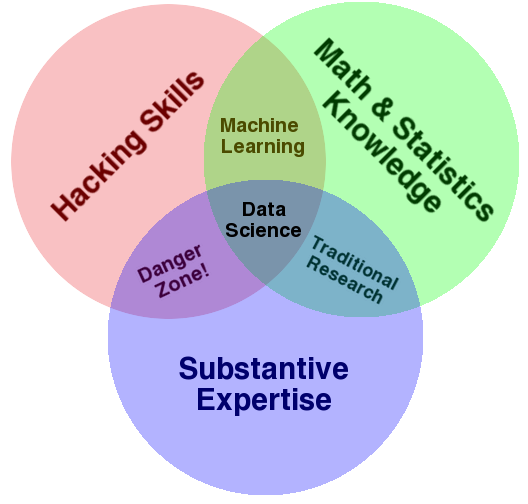
\includegraphics[scale=0.2]{figures/conway_data_science_venn_diagram.png}
  
Wir wollen Daten explorieren (=erkunden) und statistische Modelle aufstellen,\\
d.h.
  \emph{Wahrscheinlichkeitsverteilungen} modellieren.

\end{frame}

\begin{frame}
  \frametitle{Statistik? Stochastik? Was ist was?}

  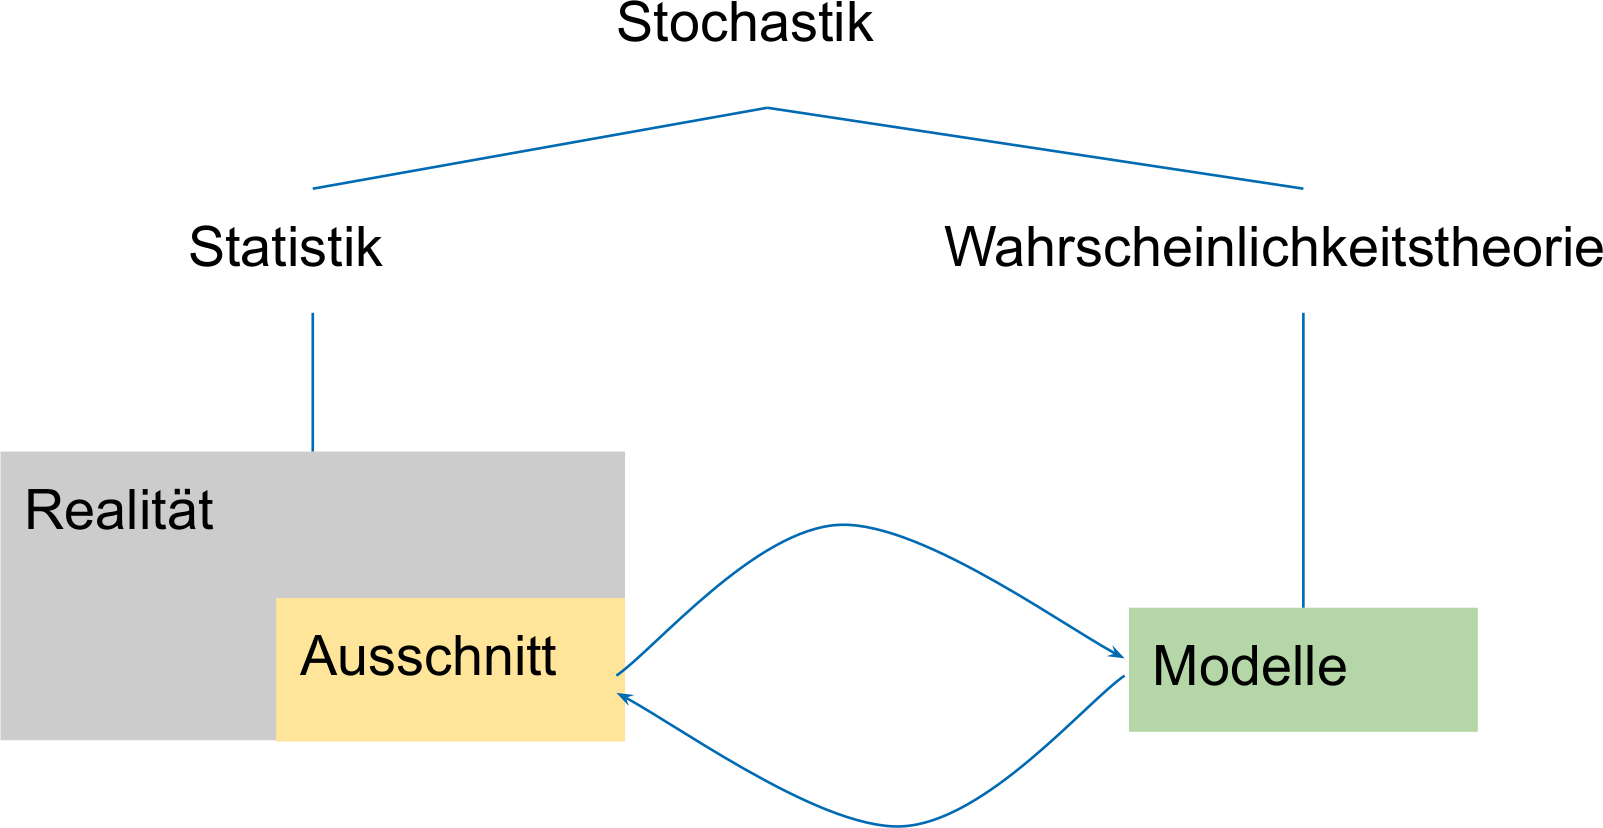
\includegraphics[scale=0.25]{figures/stochastik-ist-statistik-plus-wtheorie.png}
\end{frame}

\section{Herleitung des Wahrscheinlichkeitsbegriffs}

\begin{frame}
  \frametitle{Wie kommt man auf ``Wahrscheinlichkeit''?}

  Informatiker*innen lieben Aussagenlogik (oder?). Ein Beispiel:

  \uncover<+->{
    (Rasen ist \emph{n}ass) $\Rightarrow$ $\big($ (Es \emph{r}egnete) \quad ODER \quad (Jemand hat \emph{g}egossen) $\big)$.
    }

  \uncover<+->{
  Oder kurz, in math. Notation  $N \Rightarrow R \vee G$
} \uncover<+->{
  
  oder, in anderer Notation $(\neg N) || R || G$.
}

\vspace{1cm}
 \uncover<+->{
   Aber wie plausibel, wie glaubwürdig sind die beiden Optionen?

   \vspace{1cm}
   Regnet es oft? Hat jemals schon jemand diesen Rasen gegossen?
}
\end{frame}

\begin{frame}
  \frametitle{Plausibilität - erster Anlauf}

  Wir ordnen jeder Aussage eine Nachvollziehbarkeit (Plausibilität) zu,\\
  eine reelle Zahl, etwa

 \uncover<+->{
  \[plausi(Regen) = 20 \text{ und } plausi(Gegossen) = 5\]

Im Beispiel: wie oft wir das erlebt haben im letzten Monat.
}

\uncover<+->{
  Können wir jetzt so etwas ausrechnen?
  \[plausi(Regen\ oder\ Gegossen) =\]
}

\uncover<+->{
  Kommt drauf an. Wird manchmal gegossen, wenn es regnet?
}
\end{frame}

\begin{frame}
  \frametitle{Regeln für Plausibilitäten}
Sei $X$ eine endliche Menge von Aussagen (im Sinne der Aussagenlogik).

\uncover<+->{
  Damit eine mathematische Abbildung
  \[plausi \colon X \to \mathbb{R}\]
  sinnvoll ist, sollte wenigstens $plausi(A) = plausi(B)$ gelten, wenn $A \Leftrightarrow B$.
}

\vspace{1cm}

\uncover<+->{
  ...und weitere Logikregeln, wie z.B.

  \[plausi(A \vee B) = plausi(A) + plausi(B) - plausi(A \wedge B)\]
  }
\end{frame}

\begin{frame}
  \frametitle{Von Plausibilität zur Wahrscheinlichkeit}

\uncover<+->{
  Wir wollen den Wertebereich von $plausi$ normieren:

  \[plausi(FALSCH) = 0 \text{ und } plausi(WAHR) = 1 = 100\%\]
}

\vspace{0.5cm}

\uncover<+->{
Reicht das, um statt $plausi$ jetzt $probability$ zu sagen?
}


\uncover<+->{
  Nicht ganz. Wir benötigen z.B. auch noch
  \[plausi(A) + plausi(\neg A) = 1\]
}
\end{frame}

\begin{frame}
  \frametitle{Von Plausibilität zur Wahrscheinlichkeit}
  \framesubtitle{Cox-Jaynes-Theorem}
\uncover<+->{
  Man kann aber zeigen: es lässt sich immer so renormieren,\\ dass für eine Menge paarweiser unabhängiger Aussagen $A_1,\dots,A_n$ gilt:
  \[plausi\left( \bigvee_{i=1}^n A_i \right) = \sum_{i=1}^n plausi\left(A_i\right).\]
}

Das nennt man \emph{endliche Additivität}.
\end{frame}

\begin{frame}
  \frametitle{Aussagen? Irgendwas!}

\uncover<+->{
  Für die ``richtige'' Formalisierung von Wahrscheinlichkeit lösen wir uns noch von der Menge $X$ an Aussagen und verallgemeinern $X$ zu einer Menge von Teilmengen einer Menge $\Omega$.
}

  \vspace{1cm}

\uncover<+->{
  Sei $\Omega$ eine (beliebige) Menge, dann nennen wir die Elemente $\omega \in \Omega$ \emph{Ergebnisse}.
}

\uncover<+->{
  Jeder \emph{Menge von Ergebnissen} $A \subseteq \Omega$ würden wir eine Wahrscheinlichkeit\\
  (eine Plausibilität) zuordnen können.
}
\end{frame}

\begin{frame}
  \frametitle{Aussagenlogik und Mengenlogik}
\uncover<+->{
  Was zuvor ``oder'' $A \vee B$ war, wird nun $A \cup B$,\\
  was zuvor ``und'' $A \wedge B$ war, wird nun $A \cap B$,\\
  und aus ``Negation'' $\neg A$ wird $A^c := \Omega \setminus A := \{\omega \in \Omega \ |\ \omega \notin A\}$ (das Komplement)
}
\vspace{0.7cm}
  \uncover<+->{
    Wir identifizieren also eine Aussage mit der Menge an Ergebnissen,\\ für die die Aussage stimmt.

    Beispiel: $\Omega$ eine Menge von Zuständen, die die Welt haben kann,
    $N$ die Teilmenge aller Zustände, in denen wir sagen würden ``der Rasen ist nass'' usw.
    }
  
\vspace{0.7cm}
\uncover<+->{
  Eine Menge von Ergebnissen, der wir eine Wahrscheinlichkeit zuordnen,\\
  heißt \emph{Ereignis}.
  }
\end{frame}

\begin{frame}
  \frametitle{Wahrscheinlichkeit von Ereignissen}
\uncover<+->{
 Sei $\mathcal{F} = \{A,\ B,\  \dots \subseteq \Omega\}$ eine Menge von Ereignissen, die uns interessieren.
}

\uncover<+->{
  Mit $A,B \in \mathcal{F}$ sind auch $A \cup B$ und $A \cap B$ interessante Ereignisse!

  Auch $A^c = \Omega \setminus A$ ist interessant.
}

\vspace{0.6cm}

\uncover<+->{
  Wenn für $A,B \in \mathcal{F}$ auch $A\cup B, A \cap B$ und $A^c$ in $\mathcal{F}$ liegen,\\
  und auch $\emptyset = \{\}$ und ganz $\Omega$ Elemente von $\mathcal{F}$ sind,\\
  dann können wir mit Elementen von $\mathcal{F}$ rechnen wie mit Aussagen.
}

\vspace{0.6cm}

\uncover<+->{ 
  Wir schreiben dann die Zuordnung Ergebnismenge $\mapsto$ Plausibilitätswert als
  \[P \colon \mathcal{F} \to [0,1]\]
}
\end{frame}

\begin{frame}
  \frametitle{Definition: Ereignisraum}

  Sei $\mathcal{P}(\Omega) = \{A \subseteq \Omega\}$ die Potenzmenge (=die Menge aller Teilmengen) einer Menge $\Omega$. Dann heißt ein Mengensystem $\mathcal{F} \subseteq \mathcal{P}(\Omega)$ eine \emph{Menge von Ereignissen}, wenn
  \begin{enumerate}
  \item ``WAHR'' ein Ereignis ist: $\Omega \in \mathcal{F}$
  \item ``logisches NICHT'' von Ereignissen geht: $A \in \mathcal{F} \Rightarrow A^c \in \mathcal{F}$
  \item ``logisches ODER'' von Ereignissen geht: $A_1,\dots, \in \mathcal{F} \Rightarrow \bigcup_{i\geq 1} A_i \in \mathcal{F}$.
  \end{enumerate}

  \vspace{0.6cm}
  
  Auf mathematisch sagt man statt ``Menge von Ereignissen'' auch \emph{$\sigma$-Algebra} (sprich: Sigma-Algebra) und nennt die Elemente \emph{messbare Mengen}.
  
  Wir nennen $(\Omega, \mathcal{F})$ auch \emph{Ereignisraum}.
\end{frame}

\begin{frame}
  \frametitle{Beispiel}
\uncover<1->{ 
  Mit $\Omega = \{R,G,T\} = \{Regnete, Gegossen, Trocken\}$
  und $\mathcal{F} = \mathcal{P}(\Omega)$ können wir unser Beispiel besprechen,
  und den \emph{Elementarereignissen}
  \[\{R\}, \{G\}, \{T\} \in \mathcal{F}\]
  Plausibilitäten zuordnen,}
\uncover<2-3>{z.B.
  \[P(\{R\})=2/3,\quad P(\{G\})=1/6,\quad P(\{T\})=1/3\]
}

\uncover<3-3>{Problem 1:
  \[1 = P(\Omega) = P(\{R\}\cup \{G\}\cup \{T\}) =P(\{R\})+(\{G\})+(\{T\}) > 1\]
}

\vspace{-4cm}

\uncover<4->{also besser
  \[P(\{R\})=1/2,\quad P(\{G\})=1/6,\quad P(\{T\})=1/3\]
}

\uncover<5->{Problem 2:
  In unserer Modellierung schließen sich ``Regnete'' und ``Gegossen'' aus.
  Das passt nicht zur Realität!
  Korrekter wäre R = Regnete-aber-nicht-gegossen usw.
  }
  
\end{frame}

\begin{frame}\frametitle{Beispiel an der Tafel}
  Wir betrachten das Standardbeispiel eines Würfels (D6) an der Tafel
\end{frame}

\begin{frame}\frametitle{Definition Wahrscheinlichkeitsmaß}
  Sei $(\Omega, \mathcal{F})$ ein Ereignisraum, also $\mathcal{F}$ eine Menge von Ereignissen\\
  (sodass die Regeln ``WAHR'',``NICHT'',``ODER'' für Ereignisse gelten).

  
  Dann heißt eine Abbildung
  \[P \colon \mathcal{F} \to [0,1]\]
  \emph{Wahrscheinlichkeitsmaß}, wenn
  \begin{itemize}
    \item $P(\Omega) = 1$ (Normierung) und
    \item für paarweise disjunkte Ereignisse $A_i \in \mathcal{F}$ gilt
      \emph{$\sigma$-Additivität}:
      \[P\left( \bigcup_{i} A_i\right) = \sum_i P\left(A_i\right).\]
  \end{itemize}
\end{frame}

\begin{frame}\frametitle{Beispiel an der Tafel}
  Wir betrachten das Standardbeispiel eines \emph{fairen} Würfels (D6) an der Tafel
\end{frame}

\begin{frame}\frametitle{Definition Gleichverteilung}
  Auf einer endlichen Menge $\Omega$ mit Kardinalität $N := |\Omega|$ ist mit $\mathcal{F} := \mathcal{P}(\Omega)$ und
  \[P(A) := \dfrac{|A|}{N}\]
  ein Wahrscheinlichkeitsmaß auf $\Omega$ definiert, welches wir \emph{Gleichverteilung} nennen.
\end{frame}

\begin{frame}\frametitle{Beispiel an der Tafel}
  Wir betrachten das Beispiel eines \emph{unfairen} Würfels, der nur $6$en wirft, an der Tafel
\end{frame}


\begin{frame}\frametitle{Definition Dirac-Verteilung}
  Für einen beliebigen Ereignisraum $(\Omega, \mathcal{F})$ und ein festes Element $\xi \in \Omega$
  ist
  $\delta_\xi \colon \mathcal{F} \to [0,1]$ mit
  \[A \mapsto \begin{cases} 1 & \xi \in A, \\ 0 & \text{sonst} \end{cases}\]
ein Wahrscheinlichkeitsmaß definiert, welches wir \emph{Dirac-Maß mit Masse an $\xi$} nennen.
\end{frame}

\begin{frame}\frametitle{Ausblick}
  Nächstes Mal besprechen wir den Begriff der Zufallsvariable, klären was es mit \emph{Zufall} dabei auf sich hat, nutzen den Würfel nochmal als Beispiel und führen dann den Begriff der \emph{pmf} (probability mass function, Wahrscheinlichkeitsmassefunktion) ein, den Sie in MafIn3 vermutlich schon gesehen haben.

  Außerdem klären wir das Verhältnis Daten vs. Modell in der Sprache der Wahrscheinlichkeitsverteilungen und fangen mit dem Programmieren an.
\end{frame}

\begin{frame}[separator]
  \frametitle{Vielen Dank für Ihre Aufmerksamkeit!}
\end{frame}

\end{document}

%%% Local Variables:
%%% mode: latex
%%% TeX-master: t
%%% End:
